\section{Our process}
Our process was inspired by Essence, which is previously described in \autoref{sec:essence}.
We have been working with a ScrumBut approach in the beginning of the semester, but we decided that we wanted to try a new organization this semester, and during the courses of \textit{Software Innovation} we decided to pivot with our process.
However, we have chosen to keep sprints, stand-up meetings and retrospective meetings from Scrum as these can complement Essence.

\subsection{Roles}
We have divided the roles that we described in \autoref{sec:team-organization} between the group.
One person has the \textit{Challenger} role.
This person is accountable for prioritizing the tasks we have in our backlog.
The process of prioritizing tasks is further described in the following section.
Another person has the \textit{Anchor} role.
This person is responsible for changes to the process and is in charge of leading evaluations of the process.
The rest of the group functions as \textit{Responders}.
These are the developers of the project.
The \textit{Child} role fluctuates between members of the group.
Everyone has the possibility to add suggestions to improve an idea and give other perspectives on the project.

\subsection{Prioritizing task}
Our board on Jira can be seen on \autoref{fig:to-do-board}.
The leftmost column is the \textit{Suggested} column.
Everyone can make suggestions of tasks that they find useful for the project.
At every stand up meeting, we discuss the newly suggested tasks.
What is discussed is the definition of done, how valuable it is for the project and how time consuming it is.
The priority of a task is then calculated as $reward - time$, which is an arbitrary number to indicate how important it is.
\\\\
The Challenger then chooses the most important features from the \textit{Discussed} column, often based on the highest priority, as \textit{Chosen for Development}.
Responders then have the opportunity to take tasks from this column and move it to the next column \textit{In progress}.
When the task has been completed, reviewed and merged into develop, it is moved to \textit{Done}.
\begin{figure}[H]
    \centering
    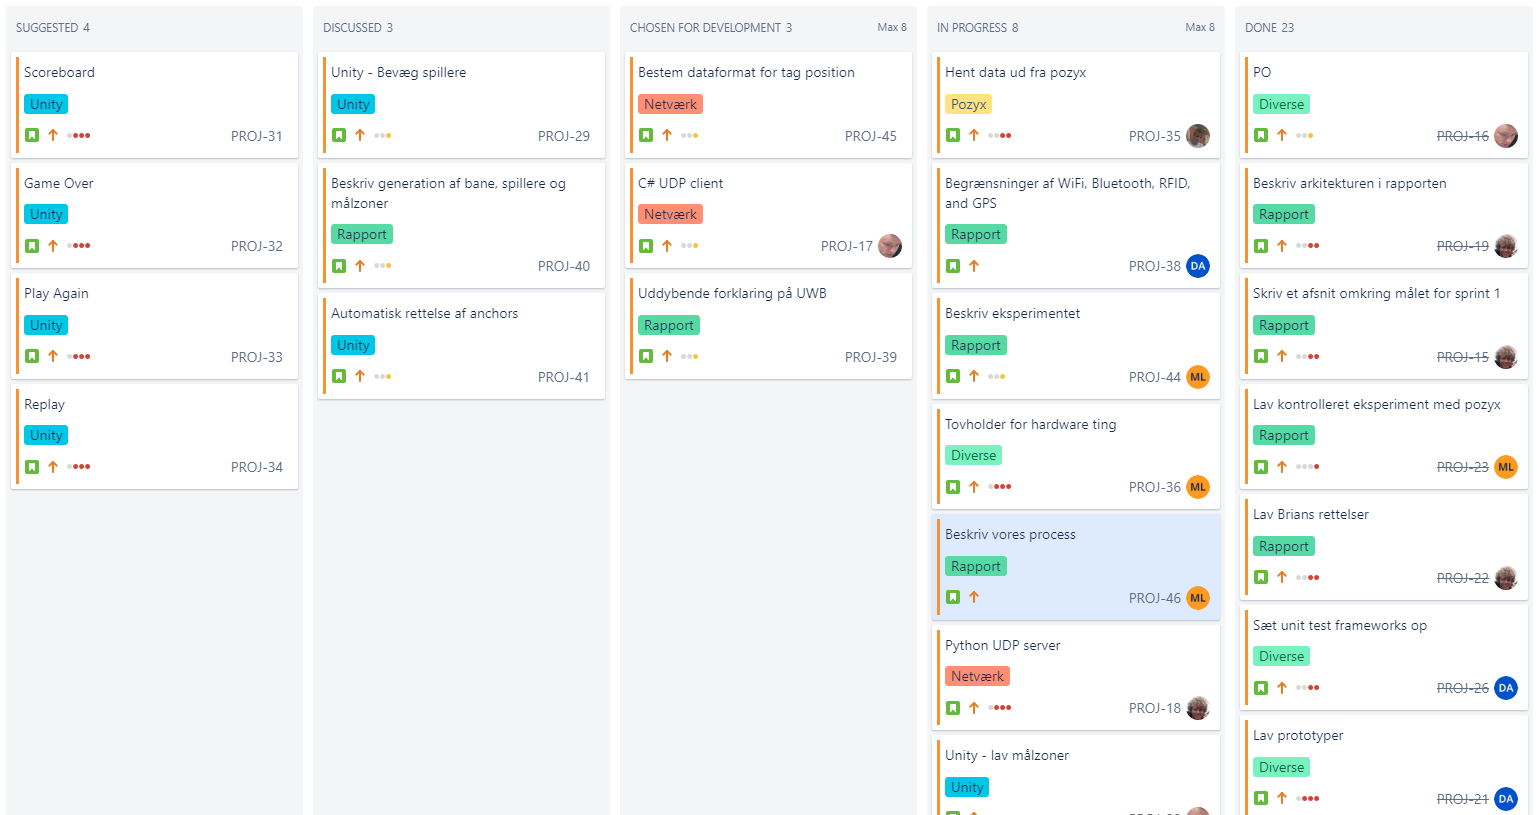
\includegraphics[width=\linewidth]{kanban.PNG}
    \caption{The board for tasks.}
    \label{fig:to-do-board}
\end{figure}

\subsection{Pair reviews}
We use pair reviews to ensure quality and make sure that people follow the test plan.
Pair reviews are also a good way to share knowledge about the implementation through the group, as people have to understand it to be able to discuss it.
Whenever a pull request has been made to develop, two people are assigned to review it.
They will review the pull request together, where they will discuss the code and ensure that the quality of it is acceptable.
On previous semesters people have reviewed the code separately, which leads to less comments as the code was not discussed between reviewers.
